\chapter{Introduction} \label{chap:intro}

%%\section{Motivation}\label{sect:thefirst}
%\begin{itemize}
%    \item The use of the RGB-D camera, the use of depth information, application: visual odometry on a quadcopter, human motion capture, 3D reconstruction.
%    \item but the depth image from consumer RGB-D camera has bad accuracy and noisy and missing data. does not contain any fine details, for instance the button on the shirt, some wrinkles on your hand, etc.
%        
%    it has been shown that with the noisy and imperfect measurements, the quality of the 3D reconstruction and the estimation of trajectory subject to. And these errors may accumulate frame by frame, leads to drift. and finally causes a loss of quality
%    \item some method tried to recover these details by fusing the depth data from multiple views~\cite{newcombe2011kinectfusion}, however, still the recovered details is very limited.
%    \item so here comes our work, we explore the intrinsic details of the object in an image, analyze the lights' positions and its corresponding influence of the shading on the object, the reflectance rate of the material on the objects.
%    \item talk a bit about SFS and PS, their basic definition: obtain the shape from an image when the light is known. 
%    \item say that combine SFS or PS with observed depth can eliminate ambiguities and has been widely used for shape or depth refinement by and it is usually formulated as an inverse problem. and nonlinearity within the normal exists in such an inverse problem, some people tries to use some nonlinear optimization to solve this problem but makes the process super slow, some others freeze the nonlinear part with the thing in the last iteration, but this sometimes leads to divergence problem. So we have a good method.
%  
%    \item say that some state-of-the-art methods need to make some strict assumptions like constant albedo, but not really in line with real world objects. Some others try to estimate the albedo by imposing some piecewise smoothness terms, but the estimation is not satisfying and the surface normal cannot be separated from the albedo. And here comes another new methods, and how good is ours
%    \item the idea of our two methods. use what as the input, first estimate what, then waht then what. {\color{red}(we explicitly estimate the incident illumination in the scene based on the reconstructed shape, make an estimate of the albedo distribution on the surface, and then use this information together with the lighting equation to recover the fine-grained structure and orientation of points on the surface. We assume a Lam- bertian model of reflection where incident lighting is given by an environment map that is parameterized in the spher- ical harmonic domain, and where surface properties are given by a spatially-varying albedo map.)}
%\end{itemize}

\section{Motivation}
With the advent of affordable RGB-D cameras, many research areas in modern computer vision, computer graphics and robotics have been boosted significantly, such as 3D modeling~\cite{sturm_etal_2013gcpr} and reconstruction~\cite{maier2014gcpr}, human motion capture~\cite{zhang2012real} and visual SLAM~\cite{engelhard2011real, kerl2013dense}, etc.
Although the low-cost commercial RGB-D sensors provide the RGB image and its corresponding depth information, the quality of depth is often not satisfactory.
%\begin{figure}[!ht]
%    \centering
%    \subfigure[RGB image]{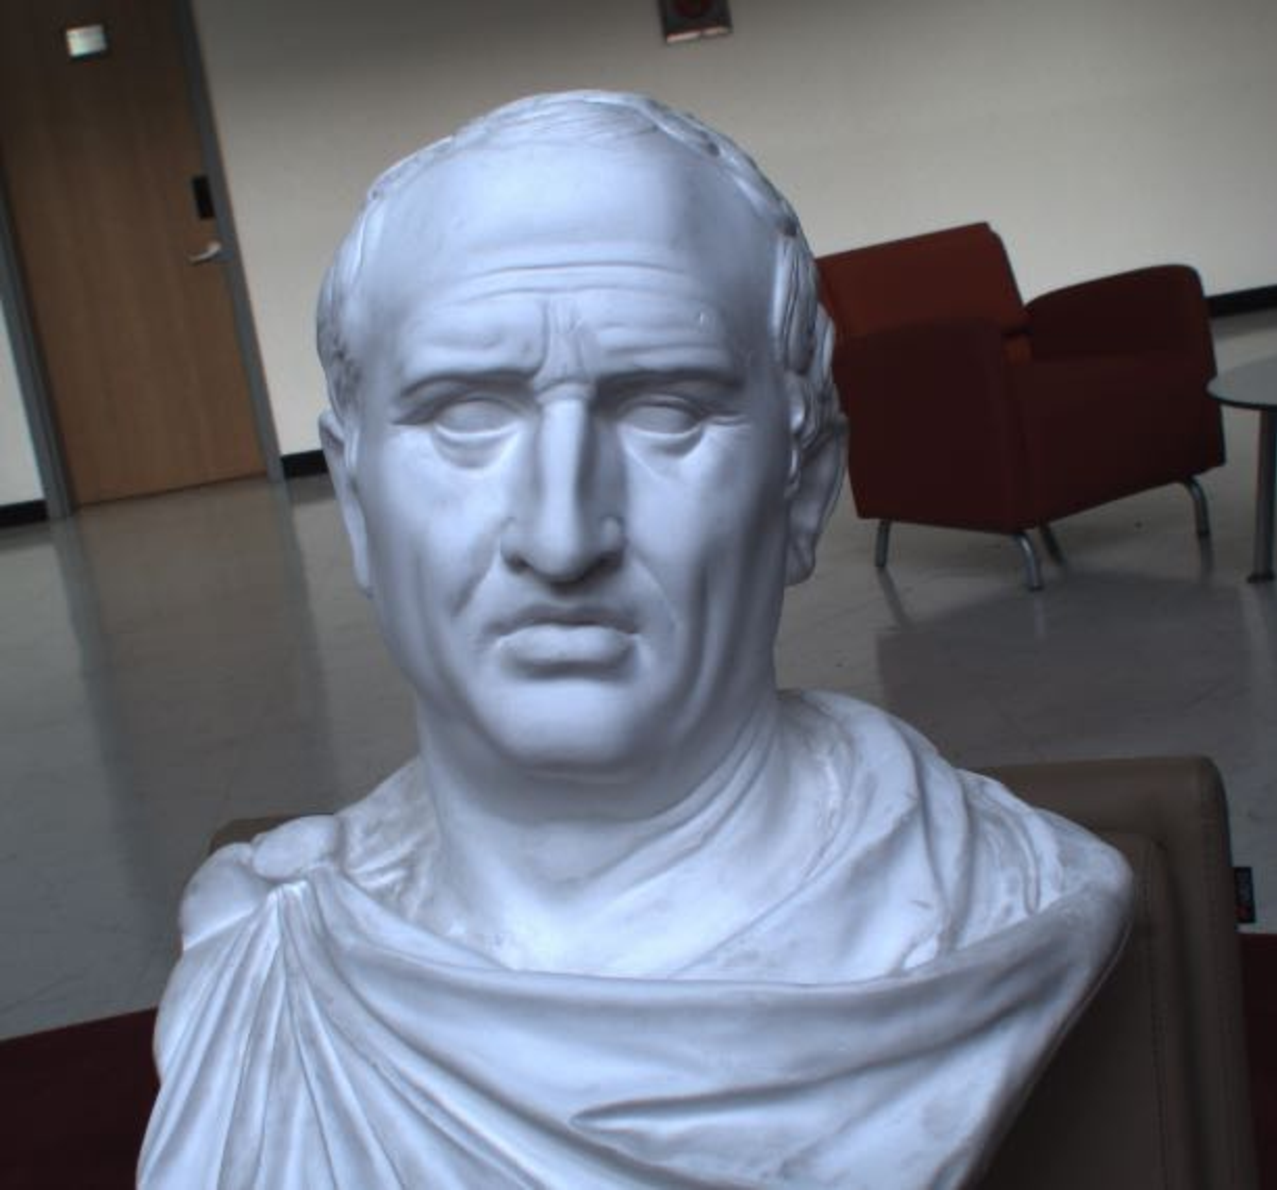
\includegraphics[width=0.28\linewidth]{figures/cicero_rgb.pdf}}
%    \subfigure[Input depth]{\label{fig:cicero_input}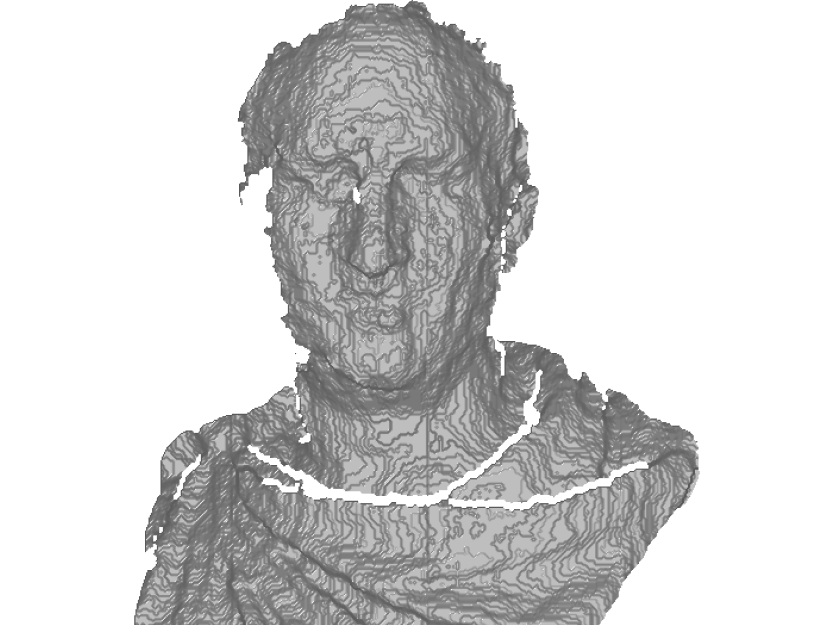
\includegraphics[width=0.32\linewidth]{figures/cicero_shape_init.pdf}}
%    \subfigure[Refined depth with our RGBD-Fusion Like method]{\label{fig:cicero_output} 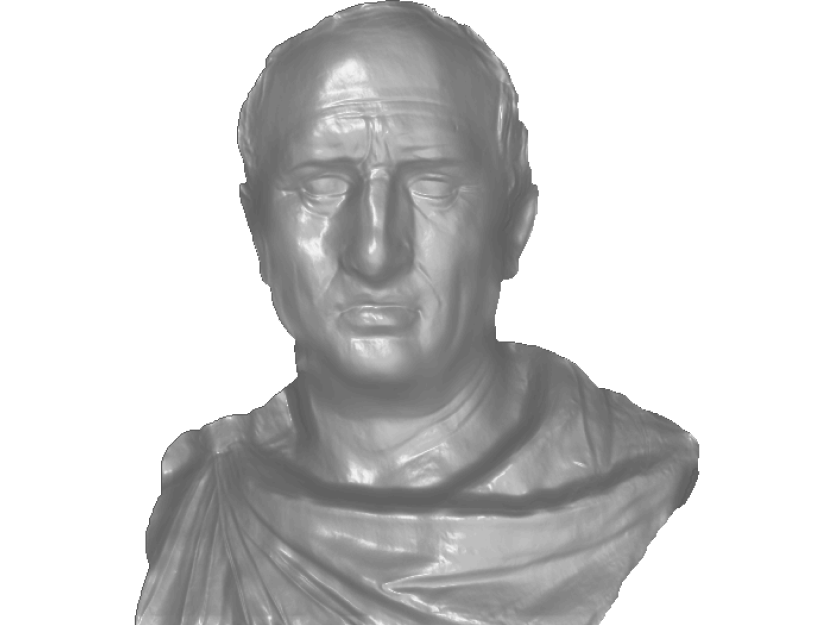
\includegraphics[width=0.32\linewidth]{figures/cicero_shape.pdf}}
%    \caption{Illustrations for the task of depth refinement. The depths are plotted as a surface for the sake of a better visualization. The RGB-D data is taken by Kinect~\cite{han2013high}.}
%    \label{fig:intro_illu}
%\end{figure}

\begin{figure}[!ht]
    \centering
    \subfigure[RGB image]{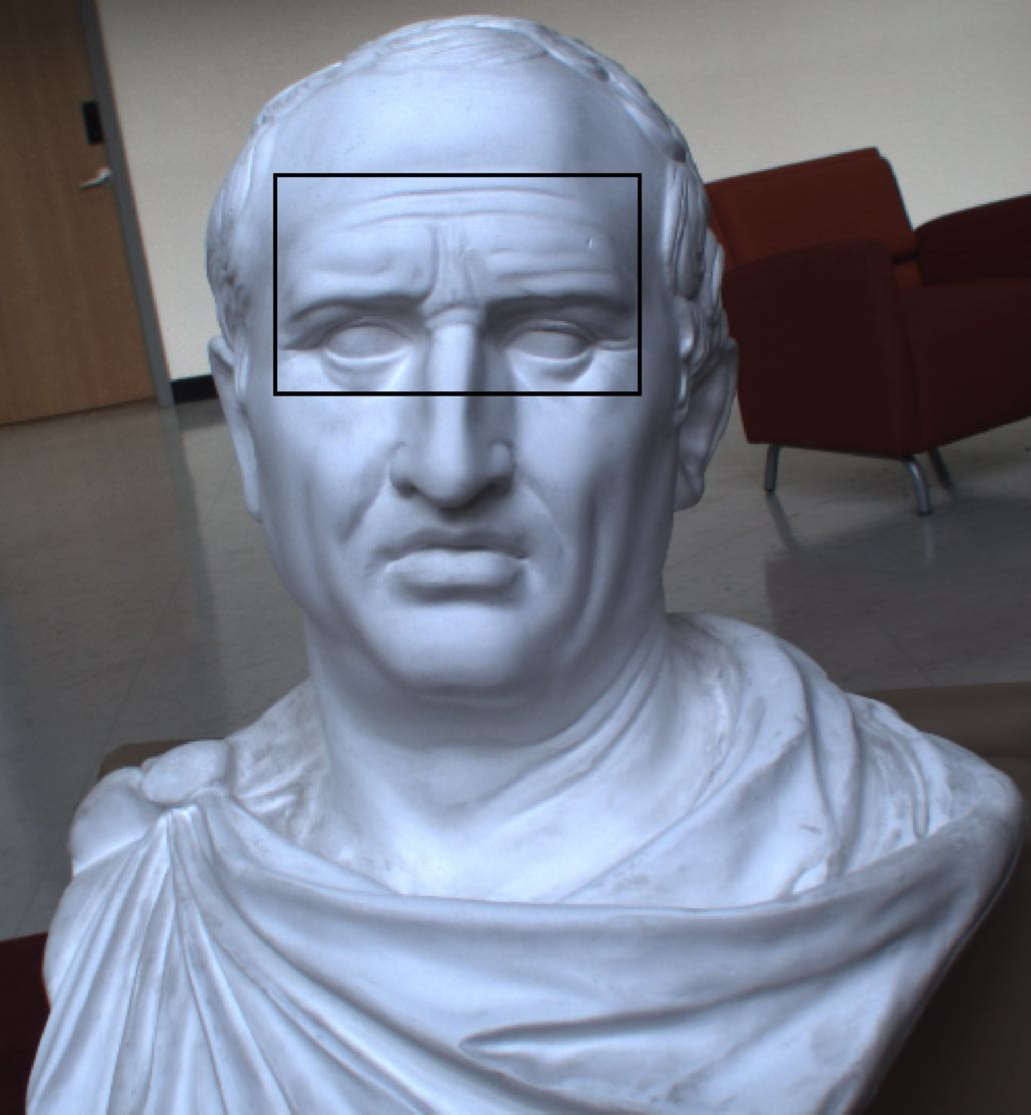
\includegraphics[width=0.25\linewidth]{figures/cicero_rgb_rec.pdf}}
    \subfigure[Input depth]{\label{fig:cicero_input}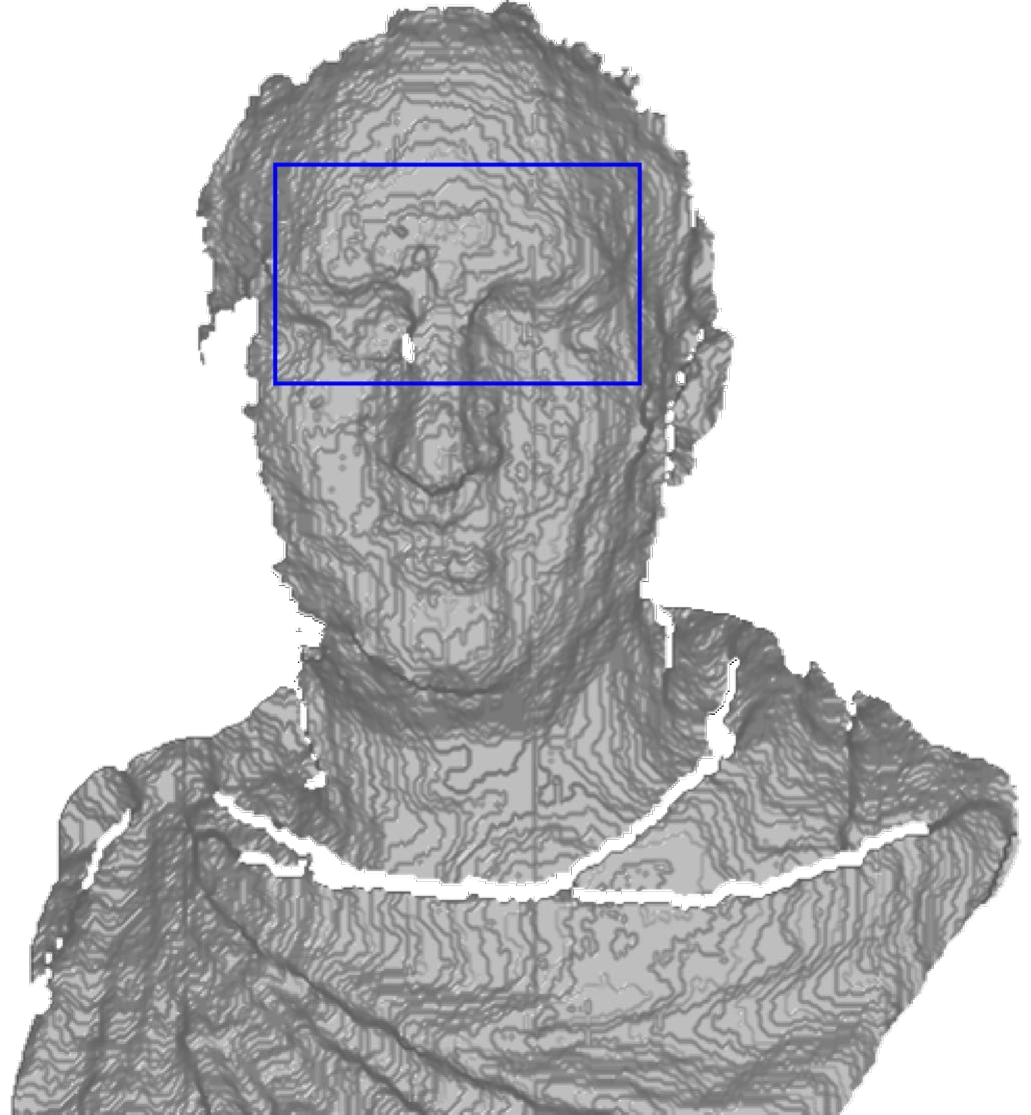
\includegraphics[width=0.25\linewidth]{figures/cicero_shape_init_rec.pdf}}
    \subfigure[Our refined depth]{\label{fig:cicero_output} 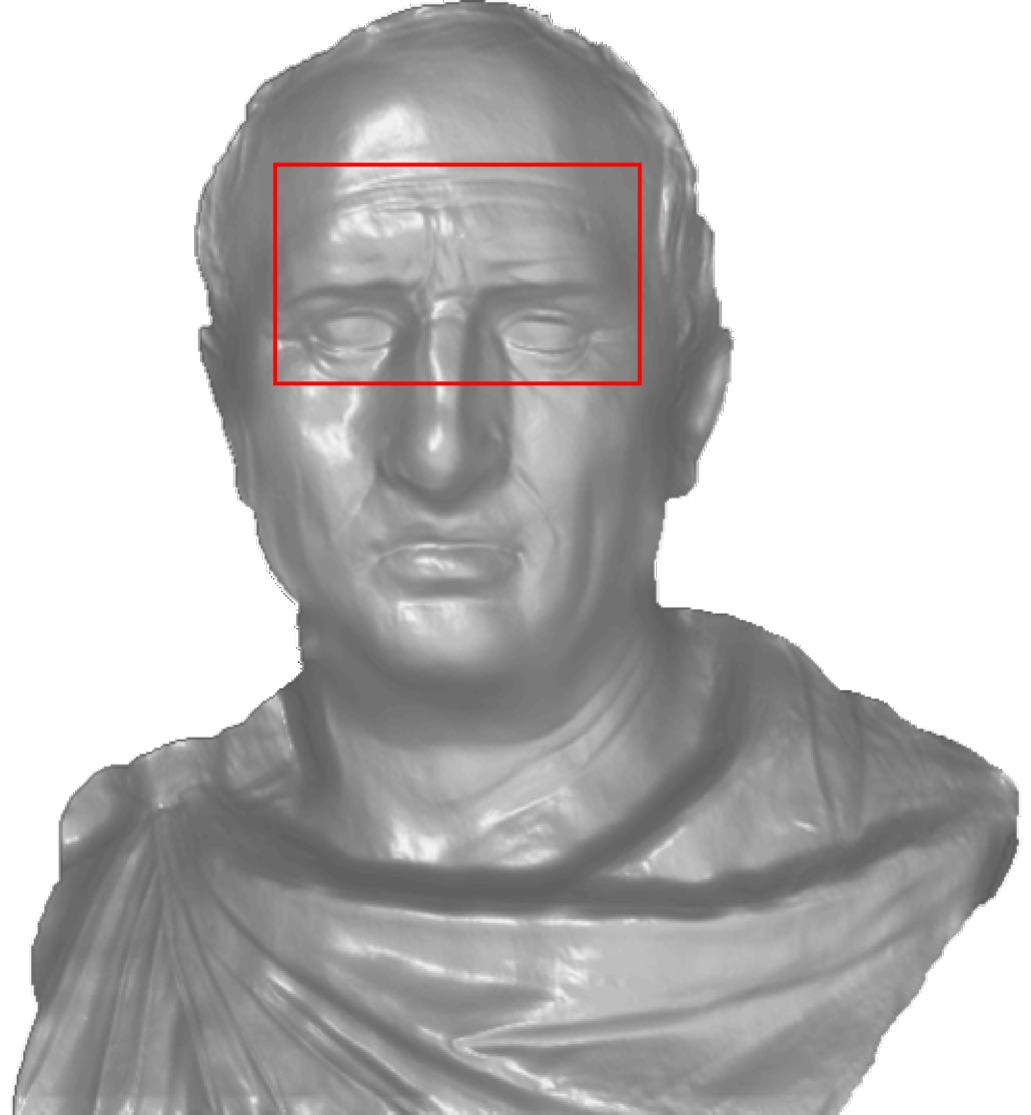
\includegraphics[width=0.25\linewidth]{figures/cicero_shape_rec.pdf}}
    \subfigure[Details]{\parbox[b]{2cm}{\label{fig:cicero_detail}
    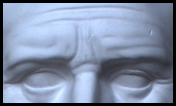
\includegraphics[width=0.14\textwidth]{figures/cicero_rgb_crop.png}\\
    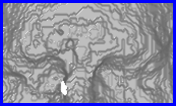
\includegraphics[width=0.14\textwidth]{figures/cicero_shape_init_crop.png}\\
   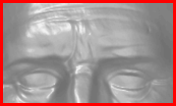
\includegraphics[width=0.14\textwidth]{figures/cicero_shape_crop.png}}}
    \caption{Illustrations for the task of depth refinement. The depths are plotted as a 3D surface for the sake of a better visualization. The input RGB and depth images are from~\cite{han2013high}. We can clearly see the improvement in the depth details using our RGBD-Fusion Like method.}
    \label{fig:intro_illu}
\end{figure}


As we can notice from Fig.~\ref{fig:cicero_input}, the depth map is very noisy and contains quantization effect with missing depth values.
Moreover, we could not see much details of the statue from the rough depth.
In contrast, Fig.~\ref{fig:cicero_output} shows the depth with much higher quality after the refinement using our approach which contributes to the preservation of geometric details.
To highlight, Fig.~\ref{fig:cicero_detail} illustrates the significant improvement in the regions of the forehead where the details of wrinkles and eyes are recovered from the raw depth. 


As a concrete example, it has been shown in~\cite{maier2013thesis} that the quality of 3D reconstruction may suffer from the noisy and imperfect depth measurements, and the estimation of camera trajectory will also drift severely because of the accumulated errors from the rough depths.
There are some methods, e.g. KinectFusion~\cite{newcombe2011kinectfusion}, which tried to recover these details by fusing all the depth data from multiple views, nevertheless, the recovered details are still very limited.
Provided we can enhance the quality of input rough depth in Fig.~\ref{fig:cicero_input} to the refined depth in Fig.~\ref{fig:cicero_output}, all the tasks which rely on RGB-D sensors can be further improved. 

\section{Problem Statement}

In this dissertation, we delve into the research of the refinement for a single depth map.
To refine the depth information from consumer depth sensors, the intrinsic details of an object should be explored with the aid of RGB image(s), such as the the positions of the scene illuminations, their corresponding influences on the object's shading, and also the reflectance (albedo) of the object's material.
Shape from shading (SFS) and photometric stereo (PS) are the fundamental approaches which can study the intrinsic properties of images, including layout patterns and geometric details. 
Therefore, they have been successfully integrated into many state-of-the-art depth enhancement methods.

These shape refinement approaches based on SFS or PS are usually formulated with the Lambertian reflectance model.
Refining the depth from this model is an inverse problem, in which nonlinearity exists. 
Some methods~\cite{wu2014real, or2016real} directly applied the nonlinear optimization algorithm like Levenberg Marquardt or the alternating direction method of multipliers (ADMM) to solve the problem which led to runtime issue. 
Other methods~\cite{or2015rgbd} froze the nonlinear part with the outcome from the last iteration to cancel out the nonlinearity.
However, such fixed-point scheme sometimes causes the optimization to diverge.
As a consequence, we propose a method called the RGB ratio model.
With the red, green and blue LED lights set up in various directions, we are able to build a lighting model for each channel of the color image acquired from RGB-D sensors.
The proposed setup and model can resolve the nonlinearity and provide a closed-form solution. 
It will be shown in chapter~\ref{chap:result} that the RGB ratio model generally achieves similar accuracy to the state-of-the-art methods and has better performance in some cases.


Furthermore, it should be mentioned that many shading-based depth refinement methods require making the assumption that the albedo is either uniform or constant~\cite{wu2011shading, han2013high, park2013multiview, haque2014high, queau2017dense}, and others impose some piecewise smoothness constraints on the albedo to make this inverse problem well-posed~\cite{or2015rgbd, or2016real, kim2015joint, wu2014real}.
These methods work well on some uncomplicated objects, for example, the statue in Fig.~\ref{fig:intro_illu}, but have the difficulty in separating the changes in the albedo from the shape when the albedo becomes complicated. This makes sense because numerous real-world objects have rather elaborate patterns and colors.
So the imposed piecewise smoothness is not commonly realistic.
Consequently, we present another novel approach called the robust multi-light method which can handle the case of very complicated albedos.
The idea is to acquire several images from various illuminations with fixed camera view, and use all the information to jointly refine light, albedo and depth iteratively.
To simulate the scenario of multiple lighting conditions, we sway a white LED light source (could be the phone flashlight) and consistently capture images. 
Compared to other methods, one main advantage of the proposed method is that no regularization term needs to be imposed, which saves much unpredictable time for the tedious process of parameter tuning.

Last but not least, since the depth maps acquired from consumer RGB-D sensors usually do not have the satisfactory resolution, we used the higher-resolution RGB images as cues and have managed to integrate super-resolution with our depth refinement method.
In this way, the final refined depth can attain the same resolution as the large RGB images with all the fine details.
We believe this is the first shading-based depth super-resolution approach.

The main contributions of this dissertation are:
\begin{enumerate}
%    \item We present a more efficient and faster implementation of an advanced depth refinement method~\cite{or2015rgbd}.
    \item We propose a new RGB ratio model to resolve the nonlinearity and achieve similar accuracy to the state-of-the-art methods.
    \item We introduce a robust multi-light method which outperforms other depth refinement approaches both quantitatively and qualitatively. Moreover, no regularization is imposed.
    \item We combine the image super-resolution with our method and present the high-quality and high-resolution depth.
\end{enumerate}


\section{Outline}
The outline of the thesis is organized as follows.
In Chapter~\ref{chap:background}, we introduce the RGB-D cameras, related knowledge about shape from shading and photometric stereo as well as the state-of-the-art depth refinement approaches.
Chapter~\ref{chap:methodology} describes the methods developed in this thesis, including a modified version of RGBD-Fusion and two proposed methods. 
Extensive quantitative and qualitative evaluations of the performance of our methods are then presented in Chapter~\ref{chap:result}.
Finally, Chapter~\ref{chap:conclusion} summarizes the developed approaches and provides the possible extensions for the future research.


